\label{pd-architektur}
\section{Architektur}
Für unsere Applikationsarchitektur haben wir das \brand{Flux}\footnote{\url{https://facebook.github.io/flux/}} Architekturpattern von \brand{Facebook} eingesetzt.\newline
Die folgenden Erklärungen wurden zu grossen Teilen aus der \brand{Flux} Dokumentation\cite{flux-docs-overview} abgeleitet.
Zu den nachfolgend beschriebenen Konzepten der \brand{Flux}-Architektur mussten für unsere Realisierung keine Anpassungen gemacht werden.
Die Beschreibungen entsprechen also unserer Implementation.\newline
\brand{Flux} ist eine Architektur, die in \gls{Frontend}-Applikationen eingesetzt wird.
Ein unidirektionaler Datenfluss ist das Grundprinzip, auf welchem \brand{Flux} aufbaut, und in welchem es sich von \gls{MVC}-Architekturen unterscheidet.
Das Pattern beschreibt folgende vier Hauptbestandteile: die Stores, die Views (oder Controller-Views), die Actions und der Dispatcher.
\begin{figure}[H]
 	\centering
 	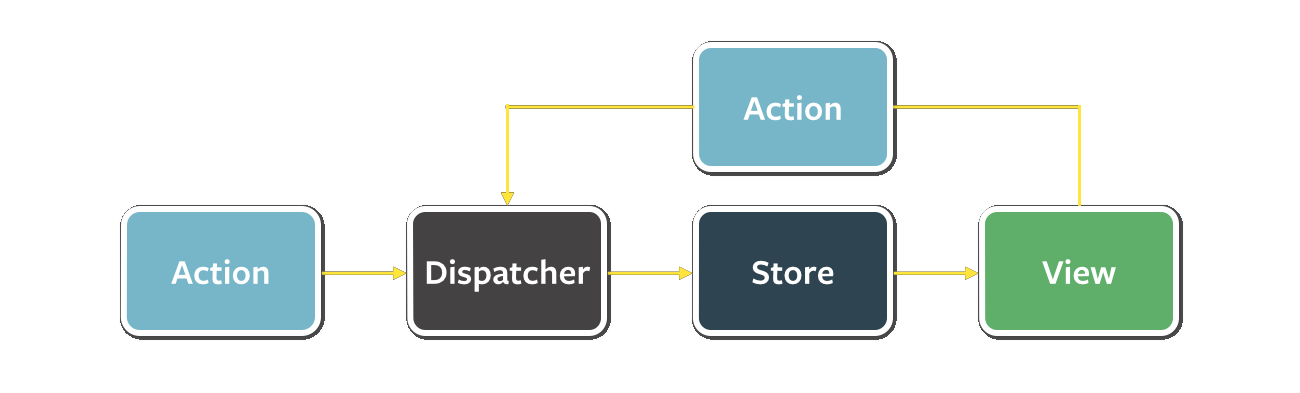
\includegraphics[width=\textwidth]{images/projektdokumentation/flux-uebersicht-weiss.png}
 	\caption{Idee der \brand{Flux}-Architektur}
 	\label{image-flux-overview-simple}
\end{figure}
\subsection{Stores}
Stores enthalten den Applikationszustand und die Applikationslogik.
Verglichen mit dem \gls{MVC}-Pattern entsprechen sie am ehesten dem Model.
Sie unterscheiden sich aber insofern, dass sie nicht unbedingt einzelne Modellklassen repräsentieren sollen, sondern domänenspezifische Aufgaben übernehmen.
Da \kort{} keine besonders komplexe Domäne enthält, ist diese Unterscheidung allerdings nicht von grosser Bedeutung.
Ein Beispiel für diese Einteilung nach Domäne und nicht nach Modell findet man in der Aufteilung von \inlinecode{UserStore} und \{inlinecode{AuthenticationStore}\newline
Stores sind als \glslink{Singleton}{Singletons} umgesetzt.
Sie registrieren sich beim Dispatcher um Updates zu erhalten und ihren Zustand entsprechend anzupassen.
Views wiederum können sich bei den Stores registrieren um neue Informationen zu erhalten, können die Stores aber nicht direkt anweisen, sich zu aktualisieren.

\subsection{Views}
Der Applikationsanwender kommuniziert seine Absichten über die View.
Deshalb gilt die View in \brand{Flux} als Auslöser für neue Aktionen.
In \brand{React} kann zwischen \emph{Views} und \emph{Controller-Views} unterschieden werden.\newline
\emph{Controller-Views} finden sich an der Spitze der View-Hierarchie.
Sie warten auf Updates der Stores und reichen die Daten entlang der Kette ihrer untergeordneten \emph{Views} weiter.\newline
Diese untergeordneten \emph{Views} wiederum reagieren auf Zustandsänderungen indem ihre \inlinecode{render()} Methode neu aufgerufen wird.
Somit bleiben \emph{View} Komponenten modular austauschbar, da sie unabhängig von ihrem Kontext eingesetzt werden können.

\subsection{Actions}
Actions sind Helfermethoden, welche im Dispatcher ein Ereignis und somit in den Stores ein Update auslösen.
Sie werden ausschliesslich durch Views ausgelöst, da diese für den Kontrollmechanismus der Applikation zuständig sind.
Ausnahmen wären hier denkbar, waren aber nicht nötig.
Beispielsweise könnte der \inlinecode{LocationStore} eine Action auslösen wenn er eine neue Position erkannt hat oder der Server wenn ein Update an die Applikation gesendet werden soll.\newline
Ausserdem sollten Daten, wenn diese für ein Update nötig sind, bereits durch die Actions an den Dispatcher mitgeliefert werden.
Aufrufe an die \gls{REST}-Schnittstelle des \glslink{Backend}{Backends} werden also über die Actions ausgelöst.
Somit kann sichergestellt werden, dass verschiedene Stores, welche auf dieselbe Action reagieren, denselben \gls{API}-Aufruf mehrmals ausführen.
In Abbildung \ref{image-flux-overview-detailed} ist dies ersichtlich.

\subsection{Dispatcher}
Der Dispatcher ist der zentrale Knotenpunkt, durch den der gesamte Datenfluss der Applikation koordiniert wird.
Seine einzige Aufgabe ist die Verteilung der Actions an die Stores.
Er enthält also keine intelligente Logik, sondern ist grundsätzlich ein Register von Callbacks.\newline
\begin{figure}[H]
 	\centering
 	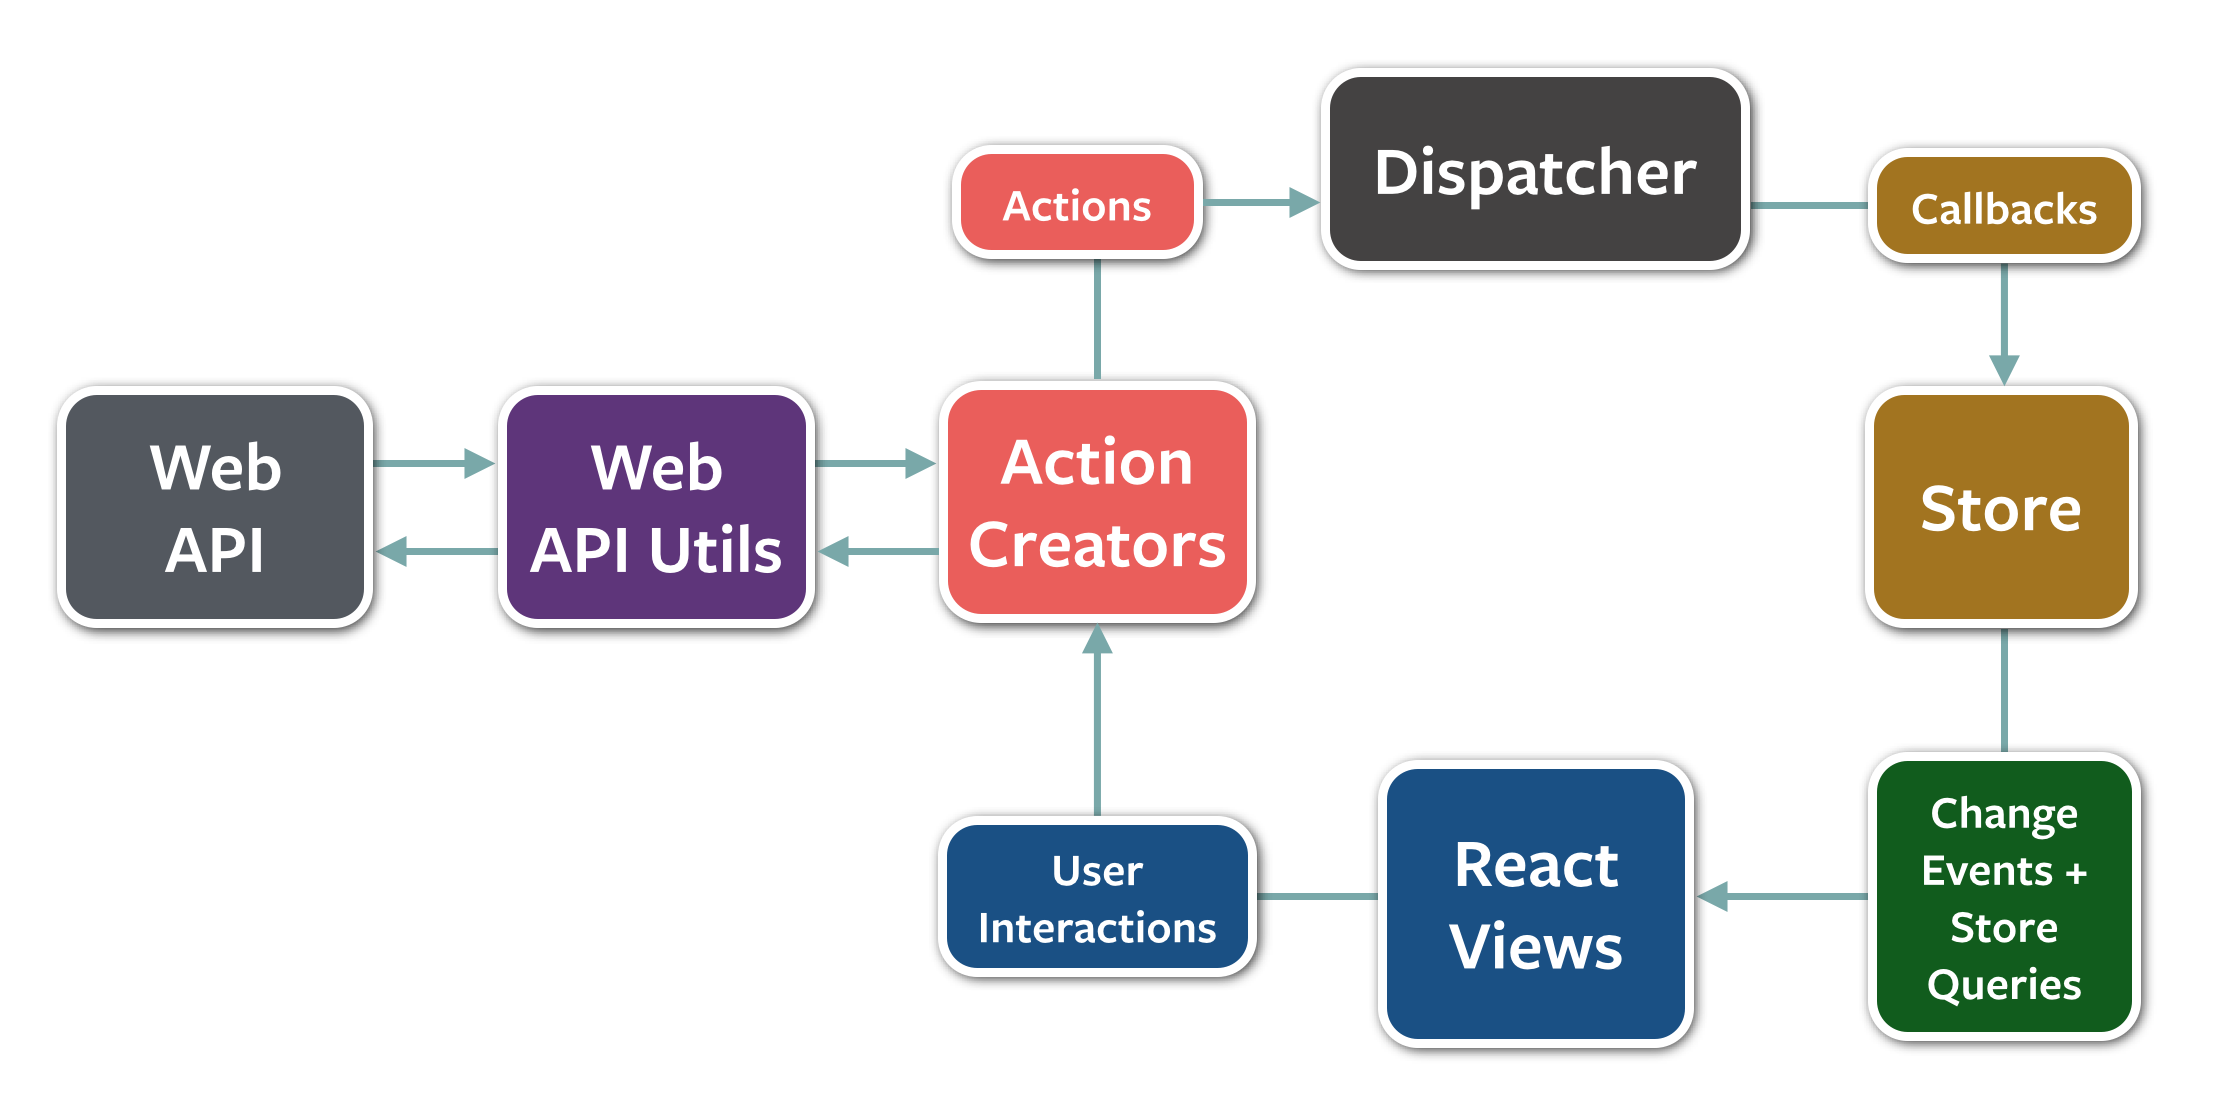
\includegraphics[width=\textwidth]{images/projektdokumentation/flux-diagram.png}
 	\caption{Vollständiges \brand{Flux}-Diagramm}
 	\label{image-flux-overview-detailed}
\end{figure}